%%%%%%%%%%%%%%%%%%%%%%%%%%%%%%%%%%%%%%%%%%%%%%%%%%%%%%%%
%%%%%%%%%%%%%%%%%%%%%%%%%%%%%%%%%%%%%%%%%%%%%%%%%%%%%%%%
%%%%%%%%%%%%%%%%%%%%%%%%%%%%%%%%%%%%%%%%%%%%%%%%%%%%%%%%
\chapter{Regression}
\label{chap:regression}

%%%%%%%%%%%%%%%%%%%%%%%%%%%%%%%%%%%%%%%%%%%%%%%%%%%%%%%%
%%%%%%%%%%%%%%%%%%%%%%%%%%%%%%%%%%%%%%%%%%%%%%%%%%%%%%%%
\section{Linear Regression (OLS)}
\label{regression:linear}

Linear regression fits the best hyperplane, or line in 1D,
to a collection of $m$ points $\mathbf{x}_{i}, y_{i}$,
typically via the method of least squares.
If $\mathbf{x}$ has $n$ features we can represent the
linear relationship between $\mathbf{x}$ and $y$ as:

\begin{equation}\label{eq:linear:one_point}
y_{i} = \beta_{0} + \sum_{j=1}^{n}\, \beta_{j} x_{ij} + \epsilon_{i}\,,
\end{equation}

\noindent where $\beta_{j}$ are the parameters of the regression
and $\epsilon$ represent random errors.
Transitioning to matrix notation\footnote{Note
that \textit{linear} regression refers to the linearity in the model parameters
$\bm{\beta}$, not $\mathbf{X}$.
The components of $\mathbf{X}_{i}$ can be, and often are,
non-linear functions of other input features.}, this is simply:

\begin{equation}\label{eq:linear:matrix}
\mathbf{y} = \mathbf{X} \bm{\beta} + \bm{\epsilon}\,,
\end{equation}

\noindent where we have set $X_{i0} =1$.
Here $\mathbf{X}$ is $m \times n$,
$\bm{\beta}$ is $n \times 1$,
and $\mathbf{y}$, $\bm{\epsilon}$ are $m \times 1$.

%%%%%%%%%%%%%%%%%%%%%%%%%%%%%%%%%%%%%%%%%%%%%%%%%%%%%%%%
\subsection{Derivation}
\label{regression:linear:derivation}

The ordinary least squares (OLS) estimate of the parameters $\hat{\bm{\beta}}$
can be found by minimizing the squares of the errors,
\ie the objective function $S\left(\bm{\beta}\right) = \norm{\bm{\epsilon}}^{2}$:

\begin{subequations} \label{eq:linear:ols}
\begin{align}
\hat{\bm{\beta}} &= \argmin_{\bm{\beta}} S\left(\bm{\beta}\right)\,, \label{eq:linear:argmin} \\
S\left(\bm{\beta}\right)
&= \norm{\mathbf{y} - \mathbf{X} \bm{\beta}}^{2} = \left(\mathbf{y} - \mathbf{X} \bm{\beta}\right)\transpose \left(\mathbf{y} - \mathbf{X} \bm{\beta}\right) \label{eq:linear:S_matrix} \\
&= \sum_{i=1}^{m} \, \abs{y_{i} - \sum_{j=0}^{n} \, \beta_{j} x_{ij}}^{2}\,. \label{eq:linear:S_components}
\end{align}
\end{subequations}

We then find the minimum of $S\left(\bm{\beta}\right)$ with respect to $\bm{\beta}$
by taking the gradient and setting it equal to zero:

\begin{subequations} \label{eq:linear:ols_derivation}
\begin{align}
S\left(\bm{\beta}\right) &=
 \mathbf{y}\transpose \mathbf{y}
-\bm{\beta}\transpose \mathbf{X}\transpose \mathbf{y}
-\mathbf{y}\transpose \mathbf{X} \bm{\beta}
+\bm{\beta}\transpose \mathbf{X}\transpose \mathbf{X} \bm{\beta} \label{eq:linear:S_expand} \\
&= \mathbf{y}\transpose \mathbf{y}
-2\, \bm{\beta}\transpose \mathbf{X}\transpose \mathbf{y}
+\bm{\beta}\transpose \mathbf{X}\transpose \mathbf{X} \bm{\beta}\,, \label{eq:linear:S_expand_simplified} \\
\partial_{\bm{\beta}} \, S\left(\bm{\beta}\right) &=
0
-2\, \partial_{\bm{\beta}} \, \bm{\beta}\transpose \mathbf{X}\transpose \mathbf{y}
+\partial_{\bm{\beta}} \, \bm{\beta}\transpose \mathbf{X}\transpose \mathbf{X} \bm{\beta} \label{eq:linear:grad_S_expand} \\
&= -2\, \mathbf{X}\transpose \mathbf{y} + 2\, \mathbf{X}\transpose \mathbf{X} \bm{\beta} = 0. \, \implies \label{eq:linear:grad_S} \\
\mathbf{X}\transpose \mathbf{y} &= \mathbf{X}\transpose \mathbf{X} \bm{\beta}\,, \label{eq:linear:penultimate}
\end{align}
\end{subequations}

\noindent where we have used\footnote{See \href{https://economictheoryblog.com/2015/02/19/ols_estimator/}{here}
and \href{https://economictheoryblog.com/2018/10/17/derivation-of-the-least-squares-estimator-for-beta-in-matrix-notation-proof-nr-1/}{here}
for the component-wise proof, but it is essentially the same as the 1D $\partial_{x} b x = b$, $\partial_{x} b x^{2} = 2 b x$.
Also note that \cref{eq:linear:S_expand_simplified} results from $\mathbf{y}\transpose \mathbf{X} \bm{\beta}$ being scalar
and thus equal to its own transpose, $\bm{\beta}\transpose \mathbf{X}\transpose \mathbf{y}$.}:

\begin{subequations} \label{eq:grad_relations}
\begin{align}
\partial_{\bm{\beta}} \, \bm{\beta}\transpose \mathbf{X}\transpose \mathbf{y} &= \mathbf{X}\transpose \mathbf{y}\,, \label{eq:grad_relations:1} \\
\partial_{\bm{\beta}} \, \bm{\beta}\transpose \mathbf{X}\transpose \mathbf{X} \bm{\beta} &= 2 \, \mathbf{X} \transpose \mathbf{X} \bm{\beta}\,. \label{eq:grad_relations:2}
\end{align}
\end{subequations}

Consequently, the optimal $\hat{\bm{\beta}}$ of \cref{eq:linear:ols}
has a closed form solution\footnote{The fitted prediction is $\hat{\mathbf{y}} = \mathbf{X} \hat{\bm{\beta}}$, with residuals $\hat{\bm{\epsilon}} = \mathbf{y} - \hat{\mathbf{y}}$.}:

\begin{equation}\label{eq:linear:betahat_OLS}
\hat{\bm{\beta}}^{\text{OLS}} = \left(\mathbf{X}\transpose\mathbf{X}\right)^{-1}\mathbf{X}\transpose \mathbf{y}\,,
\end{equation}

\noindent which is the best linear unbiased estimator (BLUE),
as can be shown with the Gauss-Markov Theorem provided
the following assumptions hold\footnote{For additional details see
\href{https://economictheoryblog.com/2015/04/01/ols_assumptions/}{here},
\href{http://people.duke.edu/~rnau/testing.htm}{here}, and
\href{https://economictheoryblog.com/2015/02/26/markov_theorem/}{here}.}:

%%%%%%%%%%%%%%%%%%%%%%%%%%%%%%%%%%%%%%%%%%%%%%%%%%%%%%%%
\subsection{Assumptions}
\label{regression:linear:assumptions}

\begin{enumerate}[noitemsep]
  \item The underlying relationship between $\mathbf{x}$ and $y$ is linear, and there are no major outliers.\label{item:regression:linear:linear}
  \item The columns of $\mathbf{X}$, \ie features, are linearly independent, \ie $\mathrm{rank}\left(\mathbf{X}\right) = n$ (no multicollinearity). This allows $\mathbf{X}\transpose\mathbf{X}$ to be inverted.\label{item:regression:linear:multicollinearity}
  \item The errors $\epsilon$ have conditional mean 0, $\expvalE{\epsilon \mid \mathbf{X}} = 0$ (exogeneity). The errors thus:\label{item:regression:linear:exogeneity}
  \begin{enumerate}[noitemsep]
    \item Have a mean of zero, $\expvalE{\epsilon} = 0$.
    \item Are not correlated with the input features, $\expvalE{\mathbf{X}\transpose\epsilon} = 0$.
  \end{enumerate}
  \item The errors are spherical, $\mathrm{var}\left(\epsilon \mid \mathbf{X}\right) = \sigma^{2} \identity$. Thus:\label{item:regression:linear:spherical}
  \begin{enumerate}[noitemsep]
    \item Each observation $\mathbf{x}_{i}$ has the same constant variance $\sigma^{2}$ (homoscedasticity).
    \item The errors are uncorrelated between observations, $\expvalE{\epsilon_{i}\epsilon_{j \neq i} \mid \mathbf{X}} = 0$ (no autocorrelation).
  \end{enumerate}
  \item The errors are normally distributed (multivariate normality)\footnote{This is not required for OLS to be the BLUE, but hypothesis testing works if true.}.\label{item:regression:linear:normality}
\end{enumerate}

If these assumptions are violated the following issues arise,
namely the model may be biased and or have a large or invalid estimated variance:

\begin{itemize}[noitemsep]
  \item[\cref{item:regression:linear:linear}.] If you are fitting nonlinear data the predictions will have large errors,
particularly when extrapolated beyond the range of the fitted data.
This will show up as systematic errors in the residuals plot,
or may be obvious when comparing observed vs predicted values.
Possible fixes include applying a nonlinear transformation to some of the features to linearize the data, \eg take the log,
adding more combinations of features, \eg higher polynomial terms,
or finding new independent features which may explain the nonlinearity.

  \item[\cref{item:regression:linear:multicollinearity}.] If some of the features are not linearly independent (multicollinearity),
they can be biasing the model and should be removed in turn until linear independence is restored.
Multicollinearity can be spotted in the input feature correlation matrix,
or if the residuals correlate to any of the features.

  \item[\cref{item:regression:linear:exogeneity}.] If something is wrong with the errors
such that they have a non-zero mean or correlate to the input features
the OLS $\hat{\bm{\beta}}$ is biased and inconsistent.
This can happen if there are omitted variables or measurement errors.
Furthermore, if $\expvalE{\epsilon \mid \mathbf{X}} = c$ only the $\beta_{0}$ intercept is affected.

  \item[\cref{item:regression:linear:spherical}.] If something is wrong with the errors
such that they have a changing variance or correlate across observations\footnote{Thus the residuals correlate with row number, \ie autocorrelation.}
the reported confidence intervals on the model parameters may be over or underestimated.
The OLS $\hat{\bm{\beta}}$ remains unbiased and has consistent coefficients, but will be biased for standard errors.

  \item[\cref{item:regression:linear:normality}.] If the errors are not normally distributed the confidence intervals are again suspect.
This can be diagnosed by comparing the errors to the normal distribution with a normal probability plot, or normal quantile plot,
or through a statistical method like the Anderson-Darling and Kolmogorov-Smirnov tests.
Note that violating normality in the errors is not as much of an issue compared to the other assumptions
since the fit will still give usable coefficients provided the assumed form of the model is correct.
Problems of this kind can arise from nonlinear data or influential outliers.
If the errors really are non-normal, a generalized linear model (GLM) could be employed to model them correctly.
\end{itemize}

%%%%%%%%%%%%%%%%%%%%%%%%%%%%%%%%%%%%%%%%%%%%%%%%%%%%%%%%
\subsection{Goodness of Fit}
\label{regression:linear:goodness_of_fit}

\subsubsection{Coefficient of Determination ($R^{2}$)}
\label{regression:linear:goodness_of_fit:R2}

The coefficient of determination\footnote{For additional details see
\href{https://economictheoryblog.com/2014/11/05/the-coefficient-of-determination-latex-r2/}{here},
\href{https://economictheoryblog.com/2014/11/05/proof/}{here}, and
\href{http://people.duke.edu/~rnau/rsquared.htm}{here}.}, $R^{2}$,
measures how much of $\mathbf{y}$'s variation is explained by the fitted model $\hat{\mathbf{y}}$,
versus by random errors $\mathbf{\epsilon}$ or other unknown sources,
as $\mathbf{y} = \hat{\mathbf{y}} + \mathbf{\epsilon}$.
$R^{2} \approx 1$ is ideal and, depending on the particular definition,
it can take values outside the typical $0 \leq R^{2} \leq 1$ range.

\begin{equation}\label{eq:regression:linear:goodness_of_fit:R2}
R^{2} = \frac{
\sum_{i=1}^{m} \left(\hat{y}_{i} - \bar{\hat{y}}\right)^{2}
}{
\sum_{i=1}^{m} \left(y_{i} - \bar{y}\right)^{2}
} = 1 - \frac{
\sum_{i=1}^{m} \hat{\epsilon}_{i}^{2}
}{
\sum_{i=1}^{m} \left(y_{i} - \bar{y}\right)^{2}
} = \rho_{y,\hat{y}}^{2}
\end{equation}

The adjusted $R^{2}$, $R^{2}_{\text{adj}}$, accounts for the degrees of freedom in the
fitted sample, $m-1$, and in the model, $m-n-1$, and is thus a better metric.

\begin{equation}\label{eq:regression:linear:goodness_of_fit:R2_adj}
R^{2}_{\text{adj}} = 1 - \frac{
\left(\sum_{i=1}^{m} \hat{\epsilon}_{i}^{2}\right)/\left(m-n-1\right)
}{
\left(\sum_{i=1}^{m} \left(y_{i} - \bar{y}\right)^{2}\right)/\left(m-1\right)
}
= 1 - \left(1-R^{2}\right)\frac{m-1}{m-n-1}
\end{equation}

\subsubsection{Standard Error of the Regression and $\chi_{\nu}^{2}$}
\label{regression:linear:goodness_of_fit:reduced_chi2}

The standard error of the regression, $s$,
and reduced \chiSqstat, $\chi_{\nu}^{2}$,
are additional ways of quantifying goodness of fit.
$s$ is a measure of the typical residual, in the units of $y$.
$\chi_{\nu}^{2}$ is a convenient way of reporting this spread in a dimensionless manner,
particularly in more sophisticated regressions where each $y_{i}$ has an \apriori estimated uncertainty, $\sigma_{i}$.

\begin{subequations}\label{eq:regression:linear:goodness_of_fit:s_red_chi2}
\begin{align}
s^{2} &= \frac{\norm{\hat{\bm{\epsilon}}}^{2}}{m-n} = \frac{1}{m-n} \sum_{i=1}^{m} \left(\hat{y}_{i} - y_{i}\right)^{2} \label{eq:regression:linear:goodness_of_fit:s} \\
\chi_{\nu}^{2} &= \frac{1}{m-n} \sum_{i=1}^{m} \frac{\left(\hat{y}_{i} - y_{i}\right)^{2}}{\sigma_{i}^{2}} \label{eq:regression:linear:goodness_of_fit:red_chi2}
\end{align}
\end{subequations}

$\chi_{\nu}^{2}$ can be interpreted as follows:

\begin{table}[H]
  \centering
  \begin{tabular}{c | p{8cm}}
$\chi_{\nu}^{2} \gg 1$ & The true model may be different than the fitted model. \\
$\chi_{\nu}^{2} > 1$ & Fit doesn't fully explain data (underfitting), or the \apriori $\sigma_{i}$ are underestimated. \\
$\chi_{\nu}^{2} \approx 1$ & Good fit! \\
$\chi_{\nu}^{2} < 1$ & Fit overexplains data (overfitting), or the \apriori $\sigma_{i}$ are overestimated. \\
$\chi_{\nu}^{2} \ll 1$ & Extreme overfitting or overestimated $\sigma_{i}$.
  \end{tabular}
%  \caption{}
  \label{table:red_chi2_interp}
\end{table}

%%%%%%%%%%%%%%%%%%%%%%%%%%%%%%%%%%%%%%%%%%%%%%%%%%%%%%%%
\subsection{Coefficient Significance}
\label{regression:linear:coeff_significance}
% TODO what is the significance of any particular \beta_{i} coefficient, via \ttest, \chiSqtest, \Ftest?? Should be able to get distribution of any \beta_{i} analytically for OLS, but can use bootstrap sampling for more complex models.

%%%%%%%%%%%%%%%%%%%%%%%%%%%%%%%%%%%%%%%%%%%%%%%%%%%%%%%%
\subsection{Ridge Regression (L2, or Tikhonov)}
\label{regression:linear:ridge}

Adding ridge (L2, or Tikhonov) regularization to OLS is much more straight forward than LASSO,
so we shall discuss it first\footnote{See \href{https://stats.stackexchange.com/a/164546}{here} for an interesting geometric explanation.}.
We wish to minimize the square errors $\norm{\bm{\epsilon}}^{2}$,
now subject to the condition that $\norm{\bm{\beta}}^{2} < t$ for some $t \geq 0$.
For any $t \geq 0$ there is a $\lambda \geq 0$ such that minimizing the following
objective function $S\left(\bm{\beta}\right)$ without conditions is
equivalent\footnote{This is sometimes termed soft-thresholding, but is really an application of Lagrange multipliers.}:
% TODo add \cref{additional:misc:opt} to Lagrange multipliers in footnote when written

\begin{equation} \label{eq:linear:ridge}
S\left(\bm{\beta}\right) = \norm{\mathbf{y} - \mathbf{X} \bm{\beta}}^{2} + \lambda \norm{\bm{\beta}}^{2}\,.
\end{equation}

After taking the gradient, we have the same terms as \cref{eq:linear:grad_S},
plus a new term\footnote{Note the similarity to \cref{eq:grad_relations:2}.} \cref{eq:linear:ridge_derivation:new}.
Rearranging \cref{eq:linear:ridge_derivation:penultimate} we can move the new term in with the old,
and quickly arrive at a modified version of the OLS solution \cref{eq:linear:ridge_derivation:betahat}.

\begin{subequations} \label{eq:linear:ridge_derivation}
\begin{align}
\partial_{\bm{\beta}} \, S\left(\bm{\beta}\right)
&= -2\, \mathbf{X}\transpose \mathbf{y} + 2\, \mathbf{X}\transpose \mathbf{X} \bm{\beta} \label{eq:linear:ridge_derivation:grad_S_repeat} \\
&+ 2\,\lambda \bm{\beta} = 0 \,\, \implies \label{eq:linear:ridge_derivation:new} \\
\mathbf{X}\transpose \mathbf{y} &= \left(\mathbf{X}\transpose \mathbf{X} + \lambda\,\identity\right) \bm{\beta} \label{eq:linear:ridge_derivation:penultimate} \\
\hat{\bm{\beta}}^{\text{ridge}} &= \left(\mathbf{X}\transpose\mathbf{X} + \lambda\,\identity\right)^{-1}\mathbf{X}\transpose \mathbf{y} \label{eq:linear:ridge_derivation:betahat}
\end{align}
\end{subequations}

%%%%%%%%%%%%%%%%%%%%%%%%%%%%%%%%%%%%%%%%%%%%%%%%%%%%%%%%
\subsection{LASSO Regression (L1)}
\label{regression:linear:lasso}

As promised, adding LASSO (L1) regularization to OLS is challenging
as the condition, $\norm{\bm{\beta}} < t$ for some $t \geq 0$,
is not differentiable, see the corners of \cref{fig:ml:l1l2:l1}, and must be dealt with carefully.
In the special case that $\mathbf{X}$ is orthonormal, $\mathbf{X}\transpose \mathbf{X} = \identity$,
a closed form solution \cref{eq:linear:lasso:betahat:1} can be derived on a case-by-case basis
at the $\beta_{i}$ coordinate-level\footnote{See \href{https://stats.stackexchange.com/questions/17781/derivation-of-closed-form-lasso-solution}{here},
\href{https://en.wikipedia.org/wiki/Lasso_(statistics)\#Orthonormal_covariates}{here},
and \href{https://xavierbourretsicotte.github.io/lasso_derivation.html}{here}.}.
In the general case, more sophisticated methods can find numerical solutions.

\begin{subequations} \label{eq:linear:lasso:betahat_all}
\begin{align}
\hat{\bm{\beta}}^{\text{LASSO}}_{j}
&= \hat{\bm{\beta}}^{\text{OLS}}_{j} \max\left(0, \frac{\lambda}{\abs{\hat{\bm{\beta}}^{\text{OLS}}_{j}}}\right) \label{eq:linear:lasso:betahat:1} \\
&= \sign{\hat{\bm{\beta}}^{\text{OLS}}_{j}} \left(\abs{\hat{\bm{\beta}}^{\text{OLS}}_{j}} - \lambda\right)^{+} \label{eq:linear:lasso:betahat:2} \\
\hat{\bm{\beta}}^{\text{OLS}}
&= \left(\mathbf{X}\transpose\mathbf{X}\right)^{-1}\mathbf{X}\transpose \mathbf{y}
= \mathbf{X}\transpose \mathbf{y} \label{eq:lasso:modified_betahat_OLS}
\end{align}
\end{subequations}

%%%%%%%%%%%%%%%%%%%%%%%%%%%%%%%%%%%%%%%%%%%%%%%%%%%%%%%%
\subsection{LASSO vs Ridge Regression}
\label{regression:linear:lasso_vs_ridge}

All the usual concepts from \cref{ml:general:reg} apply, but specifically for linear regression
both LASSO and ridge allow us to relax the multicollinearity condition.
Lasso tends to use one feature per group of correlated $\mathbf{x}_{j}$'s, setting the rest to $\approx 0$,
while ridge will keep all of the associated $\beta{j}$'s at a similar magnitude.
As one may expect from LASSO shrinking $\beta{j}$'s to zero,
it does a better job when only some of the $n$ input features infuence $\hat{y}$,
while ridge does better if most of the features have similar importances.

%%%%%%%%%%%%%%%%%%%%%%%%%%%%%%%%%%%%%%%%%%%%%%%%%%%%%%%%
%%%%%%%%%%%%%%%%%%%%%%%%%%%%%%%%%%%%%%%%%%%%%%%%%%%%%%%%
\section{Logistic Regression}
\label{regression:logistic}

Logistic regression is a simple method to create a classifier,
typically on two classes $y = 0,1$, though multinomial extensions exist.
Its name comes from the use of the logit, or log-odds, function

\begin{equation}\label{eq:logistic:logic}
l = \text{logit}\left(p\right) = \log\left(\frac{p}{1-p}\right)
\end{equation}

\noindent on the probability $p$ of class $1$.
$l$ is estimated linearly from $n$ input features $x_{j}$ with $n+1$ parameters $\beta_{j}$ as:

\begin{equation}\label{eq:logistic:logicBeta}
l = \beta_{0} + \sum_{j=1}^{n} \, \beta_{j}\,x_{j}\,.
\end{equation}

\noindent The probability $p$ is then

\begin{equation}\label{eq:logistic:p}
p = \frac{e^l}{e^l + 1} = \frac{1}{1+e^{-l}} = \text{logit}^{-1}\left(l\right)
\end{equation}

\noindent which can be turned into a predicted class through the choice of a suitable decision threshold.

The model parameters $\bm{\beta}$ are chosen by maximizing
the log of the likelihood $L$ \cref{eq:logistic:L} over $m$ known example points $\mathbf{x}_{i}, y_{i}$.
Note that $P\left(y \mid x\right)$ \cref{eq:logistic:Pr} is simply the Bernoulli distribution.
In practice the log-likelihood $\log\left(L\right)$ is maximized via gradient descent.
An example of logistic regression can be found in \cref{fig:logistic_regression_ex}.

\begin{subequations} \label{eq:logistic:L_Pr}
\begin{align}
L\left(\bm{\beta} \mid \mathbf{x}\right) &= \prod_{i=1}^{m} \, P\left(y_{i} \mid \mathbf{x}_{i};\,\bm{\beta}\right) \label{eq:logistic:L} \\
P\left(y \mid \mathbf{x}\right) &= p^y\left(1-p\right)^{1-y}, \quad y \in \{0, 1\} \label{eq:logistic:Pr}
\end{align}
\end{subequations}

\begin{figure}
\centering
% 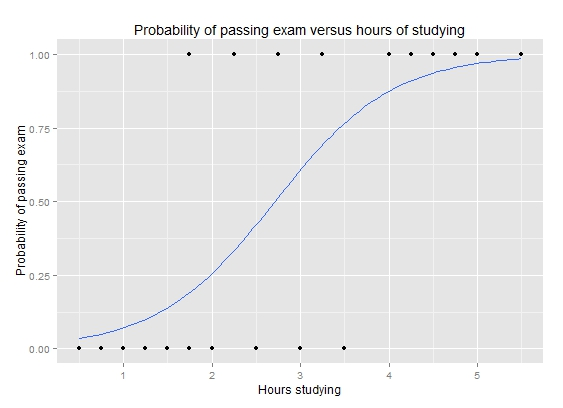
\includegraphics[width=0.8\textwidth]{figures/regression/Exam_pass_logistic_curve.jpeg}
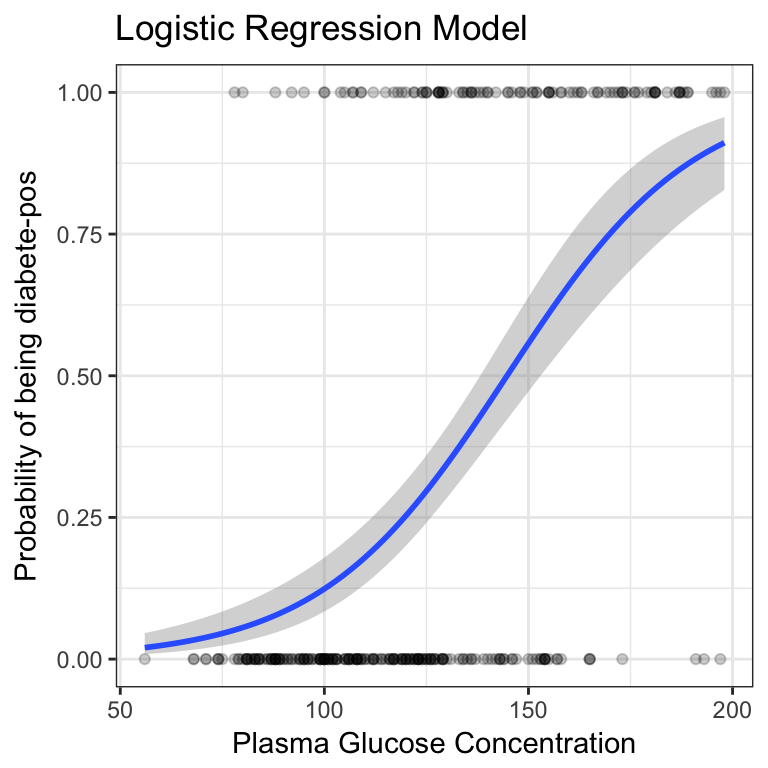
\includegraphics[width=0.7\textwidth]{figures/regression/logistic-regression-probabilities-curve.png}
\caption{
% Example logistic regression curve on one input feature, by \href{https://en.wikipedia.org/wiki/File:Exam_pass_logistic_curve.jpeg}{Michaelg2015}.
Example logistic regression curve on one input feature, by \href{http://www.sthda.com/english/articles/36-classification-methods-essentials/151-logistic-regression-essentials-in-r/}{Kassambara}.
}
\label{fig:logistic_regression_ex}
\end{figure}

% TODO any more assumptions?
Some assumptions of the logistic regression approach are:
\begin{enumerate}[noitemsep]
  \item $y$ is either present or absent (dichotomous).
  \item There are minimal correlations between the $x_{j}$ features (no multicollinearity).
  \item There are no major outliers in the data.
\end{enumerate}

% TODO pseudo R2, Wald statistic
% TODO regularized versions?
